\chapter{Implementation of cognitive radio using OpenBTS}

In our project we are able to successfully demonstrate the coexistence of 
primary users and secondary users in the GSM band. In order to accomplish this, 
implementation of a cognitive radio which detects the spectrum holes in the 
radio spectrum and enables secondary users to utilize these for communication 
is needed. An experimental setup is developed for this demonstration using 
OpenBTS and GNU radio software and USRP N210 as hardware. First a two frequency 
system is developed which is then expanded to a four frequency system.


\section{Two frequency system}

\begin{figure}
\centering
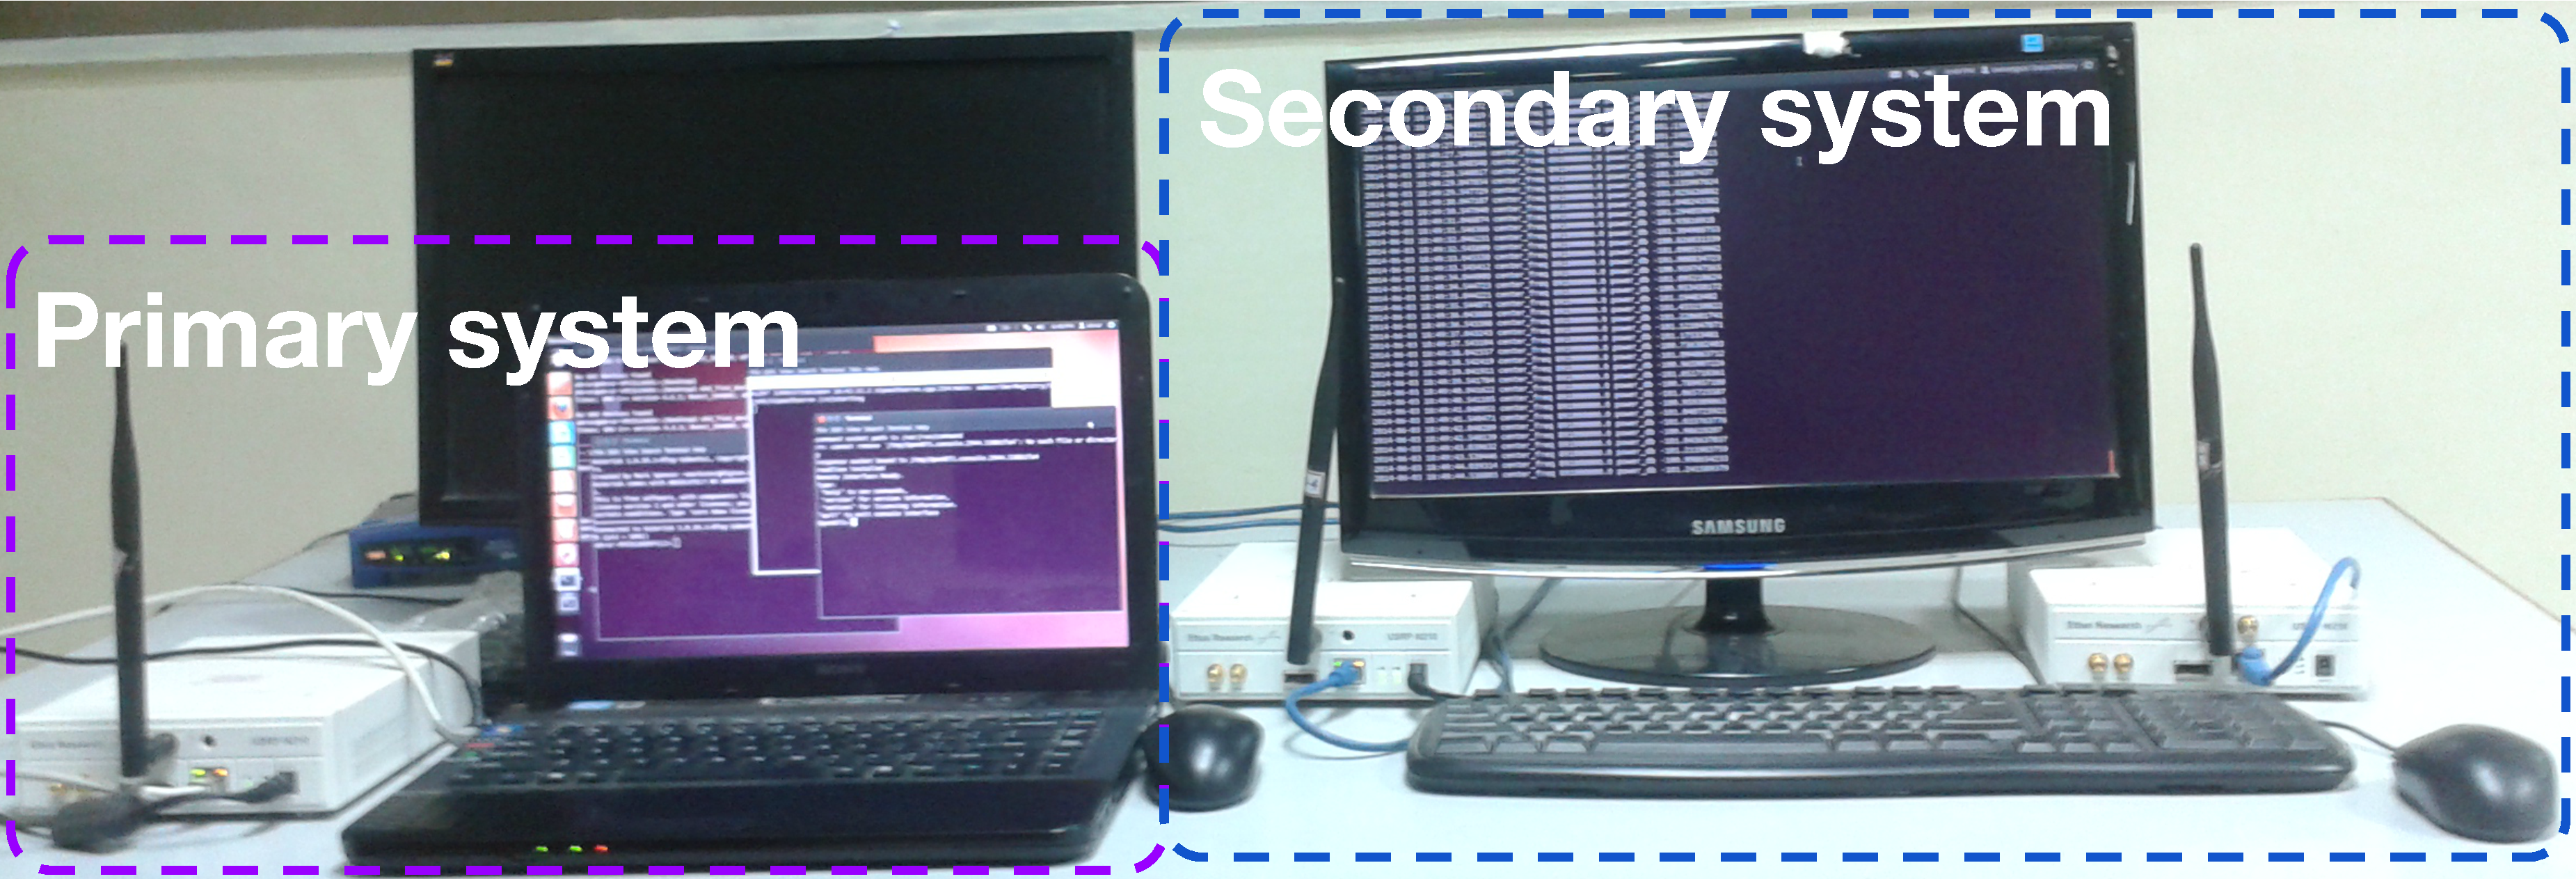
\includegraphics[width=1\textwidth]{../images/freq2}
\caption[Experimental setup, 2-frequency system]{Experimental setup of the two
 frequency system}
\label{freq2}
\end{figure}


\subsection{SYSTEM DESCRIPTION}
The figure above describes the experimental setup for two frequency system. It 
consist of one primary and one secondary subsystems. The primary subsystem has 
only OpenBTS software and one USRP for RF front. Where as secondary subsystem 
has OpenBTS along with GNU radio and two USRP kits for each of these softwares 
as hardware RF front. This secondary subsystem has cognitive capabilities. To 
provide cognitive capabilities it was necessary for OpenBTS and GNU radio to run 
together in the same computer and communicate with each other which was challenging. 
Secondary subsystem continuously senses the frequency band of interest and  
takes decision depending upon the analysis of the data collected and changes 
its parameters accordingly so that primary and secondary users coexist. The 
spectrum sensing is accomplished by using GNU radio.  GNU radio and 
OpenBTS of the secondary subsystem were made to coordinate and behave in appropriate manner and take dynamic decisions 
as and when required to make over all system behave cognitively.

\subsection{TESTING}
For two frequency cognitive system, two GSM bands are used with centre 
frequency 945MHz ($F_1$) and 950MHz ($F_2$). Secondary users are made to occupy 
one of these two bands say $F_1$. Then we make primary users enter the same 
band. This results in an increase in energy levels in this band which is sensed 
by the secondary subsystem as it is continuously scanning this band. 
Immediately secondary users are shifted to other frequency band ($F_2$) thereby 
vacating $F_1$ for primary users. Hence a two frequency cognitive system 
demonstrating coexistence of a pair of primary and secondary users is 
accomplished. 
The whole technique is described using a flow graph shown in figure
\ref{freqSys2}:

\begin{figure}[!h]
\centering
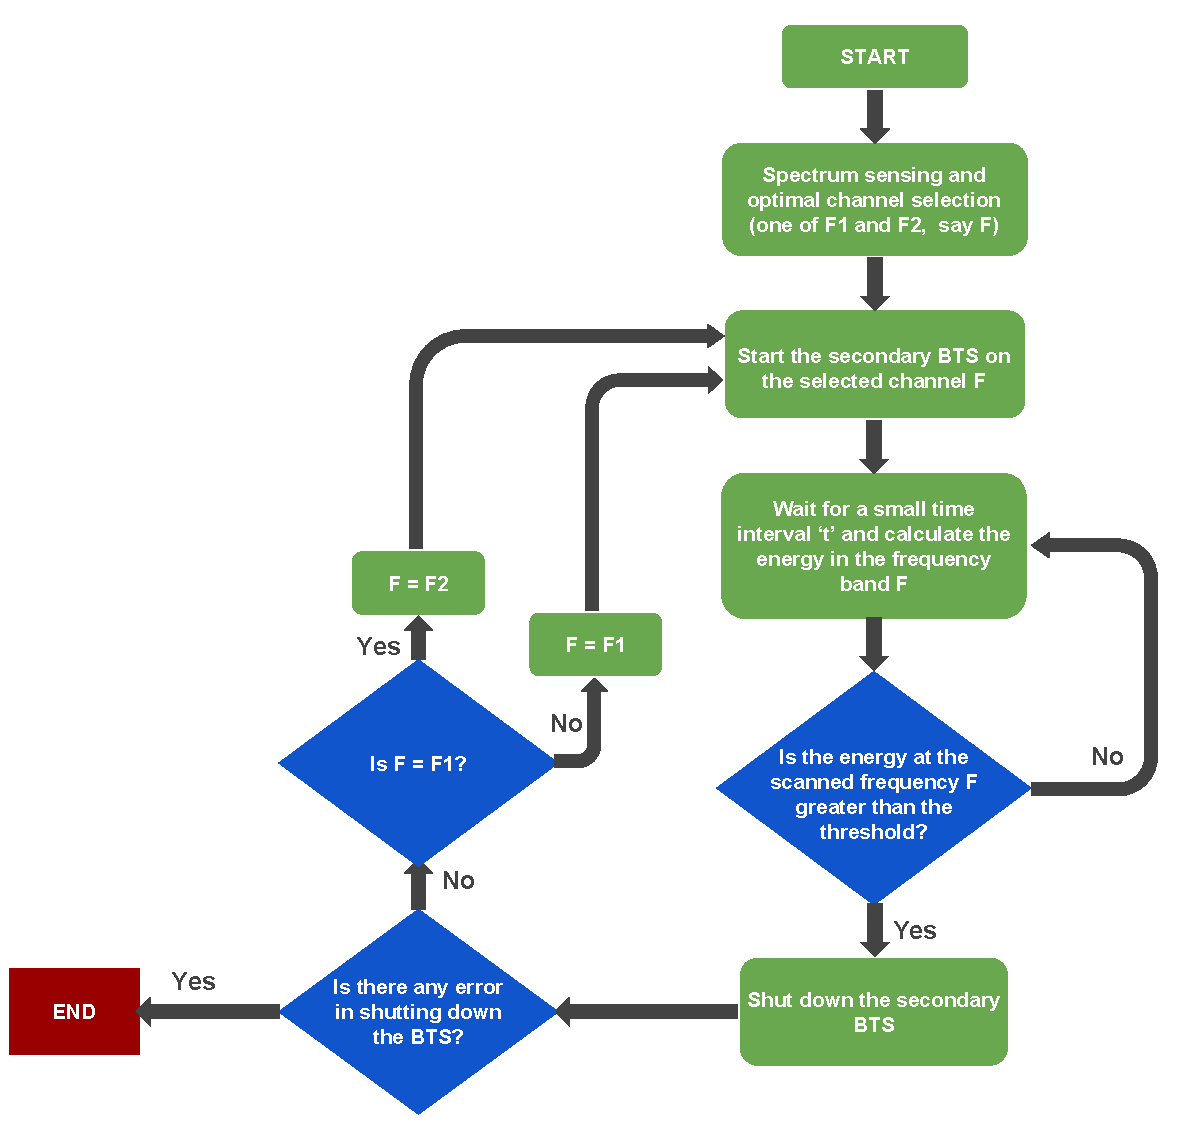
\includegraphics[width=1\textwidth]{../images/freqSys2}
\caption[Two frequency system]{Flowchart for two frequency system}
\label{freqSys2}
\end{figure}

\section{Four frequency system}
The two frequency system is expanded to a four frequency system by adding 
another primary subsystem to the two frequency experimental setup and having 
a four frequency radio spectrum instead of two. 


\begin{figure}
\centering
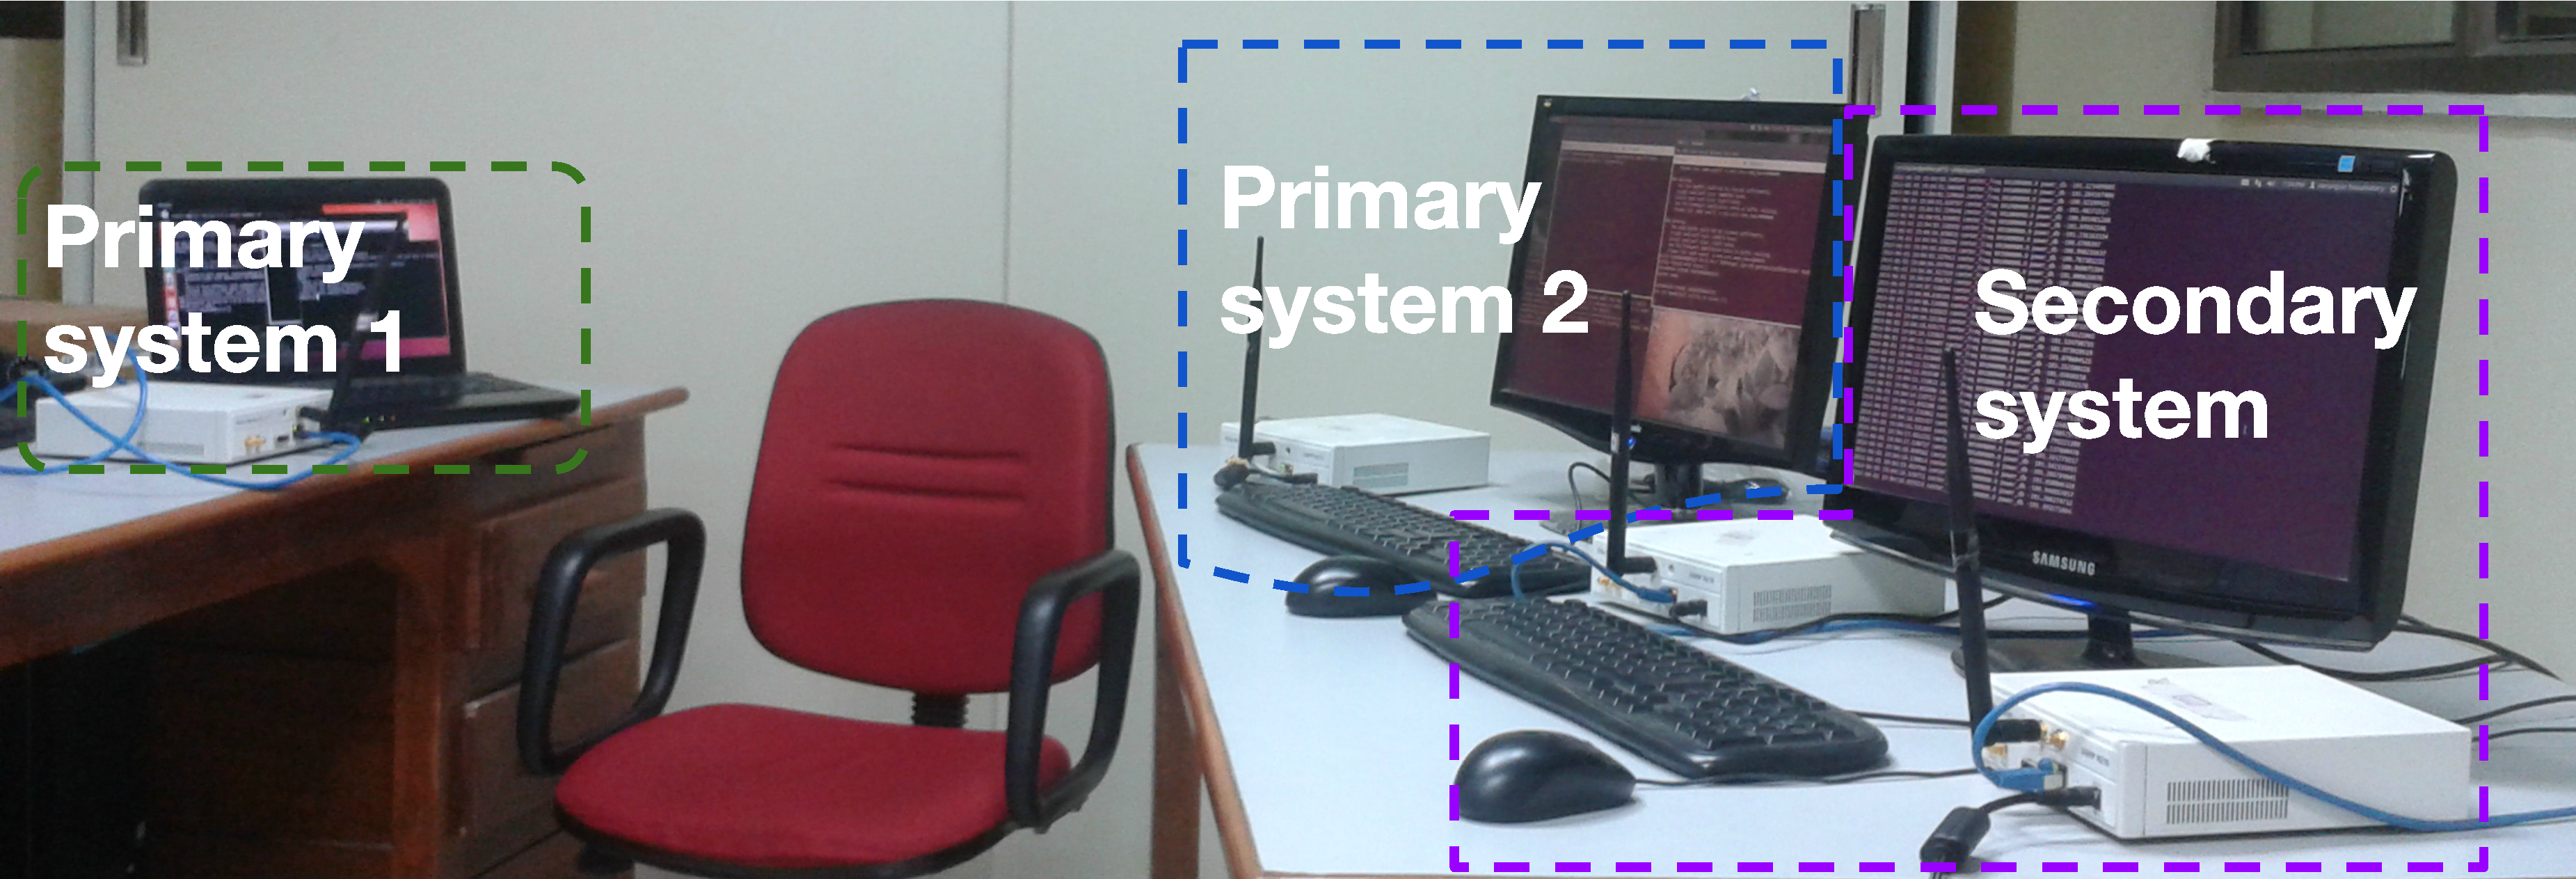
\includegraphics[width=1\textwidth]{../images/freq4}
\caption[Experimental setup, 4-frequency system]{Experimental setup of the four
 frequency system}
\label{freq4}
\end{figure}

\subsection{SYSTEM DESCRIPTION}
 The experimental setup of the four freqency system has 
has two primary subsystems and one secondary subsystem as described in the figure above. Primary subsystem 
has OpenBTS and one USRP kit and secondary subsystem has OpenBTS and GNU radio 
software and two USRP kits as we had previously in two frequency system. 
Here we have four GSM bands with centre frequencies 
$F_1$=936MHz, $F_2$=943MHz, $F_3$=950MHz, $F_4$=957MHz as the radio spectrum.
 



\subsection{Testing}
Here we make one pair of primary users occupy one of the four frequencies say 
$F_2$. We make secondary users use one frequency say $F_1$. Now other pair of 
primary users are made try and enter frequency $F_1$ for communication. This is sensed by 
the secondary system and it tries to migrate secondary users to $F_2$ which is 
also occupied. Our secondary system detects that $F_2$ is occupied and therefore 
continues to find a spectrum hole in a four frequency spectrum. It finds that 
frequency $F_3$ is unoccupied and thus allows secondary users to enter $F_3$ 
and utilize it for communication. The difference between a four frequency 
system and a two frequency system is that in a four frequency 
system the secondary subsystem has to first confirm absence of primary users 
in the band before making secondary users migrate to that band . This was not
the case in two frequency system as it has only one 
pair of primary users. Hence the other band where secondary users will be made 
to migrate is always unoccupied at the time of switching secondary radio to 
that band. So there is no need to check for the peresence of primary users in that band.

The flow graph in figure \ref{freqSys4} describes the four frequency cognitive system:

\begin{figure}
\centering
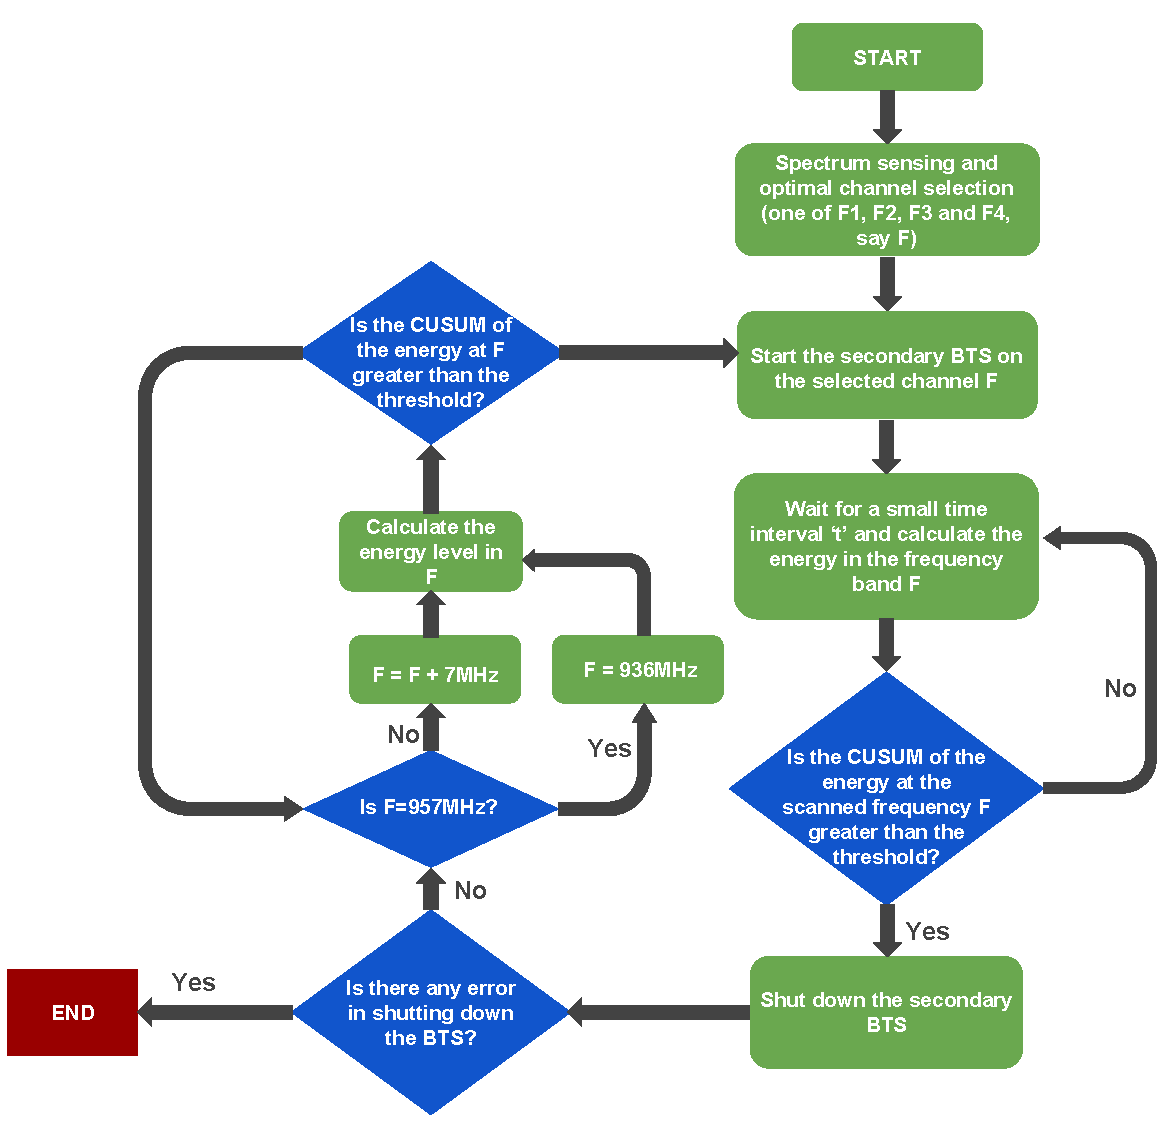
\includegraphics[width=\textwidth]{../images/freqSys4}
\caption[Four frequency system]{Flowchart for four frequency system}
\label{freqSys4}
\end{figure}

The spectrum sensing is done by energy detection technique and it was required 
that a proper threshold is set for decision making. A number of readings were 
taken to decide the noise level, energy level when only primary users are 
occupying and also energy levels when both primary users and secondary users 
exist in the same band for a short duration of time. The threshold value 
depends on the power transmitted by the users and their distance from the USRP 
kits which is RF front for GNU radio. This distance dependency can be removed by 
setting the threshold much lower so that even if the users move 
far away, the decision making is not affected.  





\section{CUSUM}
CUMSUM peak detection is also applied after energy detection to ensure that the
detected high energy in the band of interest is not due to some irrelevant 
reasons like random fluctuations in noise power etc, but due to the presence of 
primary radio in that band. This ensures high accuracy in primary radio 
detection and correct decision making.
CUSUM is basically a sequential analysis technique to detect change. 
It is a criterion for deciding when to take corrective action. As the name 
implies CUSUM involves calculating cumulative sum. This makes it sequential. 
The samples from a process $x_n$  are assigned weights $\omega_n$  and summed 
as followed,

\begin{align}
S_0 &= 0; \nonumber \\
S_{n+1} &= max(0, S_n + x_n - \omega_n) \nonumber
\end{align}
When the value of $S$ exceeds a certain threshold value a change in value has 
been found. This formula detects change only in positive direction. To detect 
change in negative direction we have to do min operation instead of max 
operation and the change  is detected when value goes below the threshold.







\section{Tasks undertaken over the year}
The next section of this chapter gives a step by step description of the tasks we 
accomplished during our project tenure. 

\begin{enumerate}

\item We began by exploring what cognitive radio is and how it can be used 
in the already existing radio. We did a literature survey on the ongoing work in the
field of cognitive radio.

\item We learned how to use the GNURadio software package starting from its installation procedure. We 
also designed an FM receiver using GNURadio Companion to get used to the software. 
Also we tried and learnt the codes of already existing signal processing blocks 
that GNU Radio provides.

\item GNURadio applications are primarily written in the Python programming 
language and hence we learned the language, Python.

\item USRP N210 kit is used as hardware in our project. We got used to this kit and 
also carried out range testing of this kit to ensure distance is not a major factor in 
our decision making algorithm and can be neglected.
\item The next task was to understand the working of OpenBTS software. Starting 
with the installation of this software we registered our GSM SIM cards in the 
local network established by OpenBTS. We could perform calling and sending SMS
between our phones using the local network established by OpenBTS with USRP 
kit as its radio interface.
\item Since spectrum sensing is major part of cognitive radio, literature survey 
on various spectrum sensing techniques was done. We chose energy detection 
spectrum sensing technique for our project and so we did detailed study of a 
technique called Average Periodogram Analysis to implement this method. We also 
simulated this technique in Matlab using various windowing methods and 
understand results. 
\item After all this the problem statement was designed and a flow graph of 
how this problem will be approached was constructed. We also decided upon the 
experimental setup required for this problem. Detailed discription of all this
is included in the previous sections of this chapter. 
 
\item  First key step to approach the problem was to run Open BTS and GNU 
Radio together in the same computer with two USRP kits connected one for 
OpenBTS and the other for GNURadio. It was a little tricky because we had to
find out whether it was possible to run two USRP kits on the same computer simultaneously.
Fortunately, it turned out it was possible if the two kits had two different IP addresses.
We then tried to figure out how to burn a different IP address to a USRP kit and
managed to do the same.
\item The next step was to build a two frequency cognitive system with a pair of 
primary and secondary users communicating in parallel and primary pair having 
higher priority when ever both try to use same radio band. Detailed description 
is in the previous sections of this chapter.
\item This two frequency system was expanded to four frequency system with two 
primary pair of users and one secondary pair of users coexisting. This 
demonstrated that both primary and secondary users can exist in the same GSM 
Network without affecting the existing system.
\end{enumerate}